
Ce chapitre représente le point de départ de mon travail. Dans ce chapitre, j'analyserai et spécifierai les besoins du projet, puis j'identifierai les différents acteurs impliqués. Ensuite, je procéderai à un benchmark des solutions disponibles et à une étude conceptuelle pour définir les besoins et les référentiels de sécurité nécessaires.

\section{Périmètre du projet}
\subsection{Contexte et justification}
Le projet \textbf{Audit365 Manager} trouve son origine dans le besoin d'Exakis Nelite d'optimiser et de moderniser ses processus d'audit et de gouvernance des \textbf{SI} Microsoft 365 (\textbf{M365}). Actuellement, les audits sont réalisés de manière manuelle, ce qui est non seulement chronophage mais aussi sujet aux erreurs humaines. La problématique principale est donc de développer une solution qui puisse automatiser et industrialiser ces processus d'audit pour garantir une meilleure efficacité et fiabilité.

\subsubsection{Audit et gouvernance}

L'audit et la gouvernance sont des concepts clés pour assurer la sécurité et le bon fonctionnement des systèmes d'information.

\textbf{Audit} : L'audit consiste à examiner attentivement les systèmes pour vérifier qu'ils respectent les règles et les normes de sécurité. Cela inclut l'inspection des paramètres, la détection des problèmes potentiels et la génération de rapports avec des recommandations pour améliorer la sécurité.

\textbf{Gouvernance} : La gouvernance implique l'établissement de règles et de processus pour gérer les systèmes de manière efficace et sécurisée. Elle assure que les systèmes sont utilisés de manière appropriée et conforme aux objectifs de l'organisation et aux réglementations.

En résumé, l'audit vérifie que tout fonctionne correctement et en toute sécurité, tandis que la gouvernance définit comment les systèmes doivent être gérés pour rester sûrs et efficaces.


\subsection{Objectifs principaux}
\begin{itemize}
    \item[•] \textbf{Développer une interface d'administration} pour les scripts d'audit, facilitant ainsi leur gestion et leur exécution.
    \item[•] \textbf{Industrialiser les processus d'audit} d'une partie ou de la totalité d'un SI collaboratif \textbf{M365}, permettant une automatisation des audits et une réduction des erreurs.
    \item[•] \textbf{Améliorer la qualité des audits} en fournissant des rapports détaillés et des recommandations de sécurité basées sur des analyses comparatives avec des baselines reconnues.
\end{itemize}

Nous travaillons déjà sur une première version de la solution qui se concentre principalement sur les services \textbf{M365} Sharepoint et Onedrive, en particulier sur SharePoint et OneDrive. Le périmètre des services Microsoft à auditer est présenté ci-dessous :

\begin{figure}[H]
    \begin{center}
        \fbox{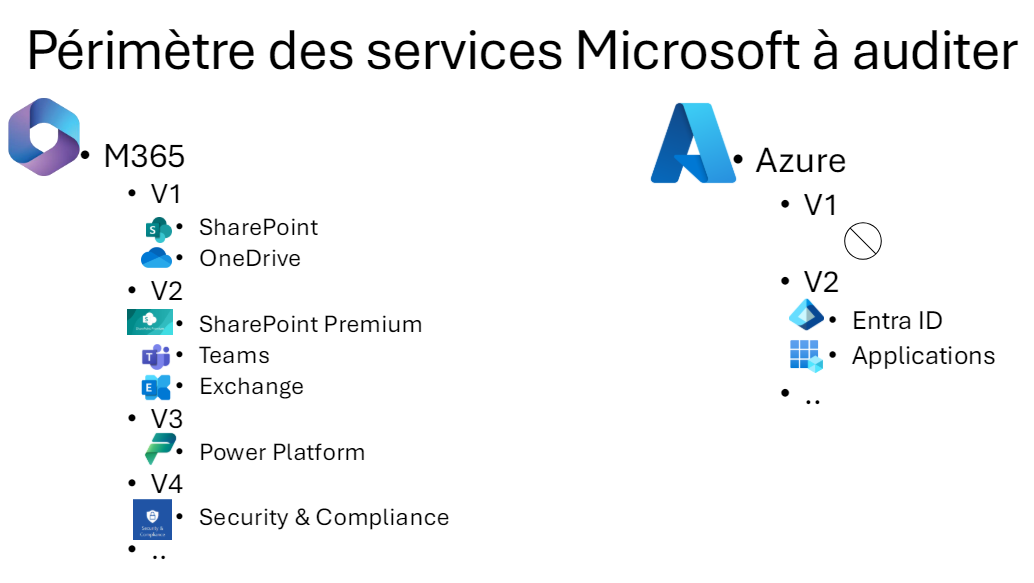
\includegraphics[scale=0.5]{images/PerimetreServices.png}}
        \caption{Périmètre des services Microsoft à auditer}
    \end{center}
\end{figure}

Cette première version (V1) inclut SharePoint et OneDrive sous \textbf{M365}. Les versions futures (V2, V3, V4) s'étendront à d'autres services tels que SharePoint Premium, Teams, Exchange, Power Platform, et les services de sécurité et de conformité. En parallèle, l'audit des services \textbf{Azure} commencera avec la version V2, incluant Entra ID et les applications.

Pour illustrer ces objectifs, le processus d'audit peut être visualisé ci-dessous ou on détaille les étapes clés de la collecte des données jusqu'à la remédiation :

\begin{figure}[H]
    \begin{center}
        \fbox{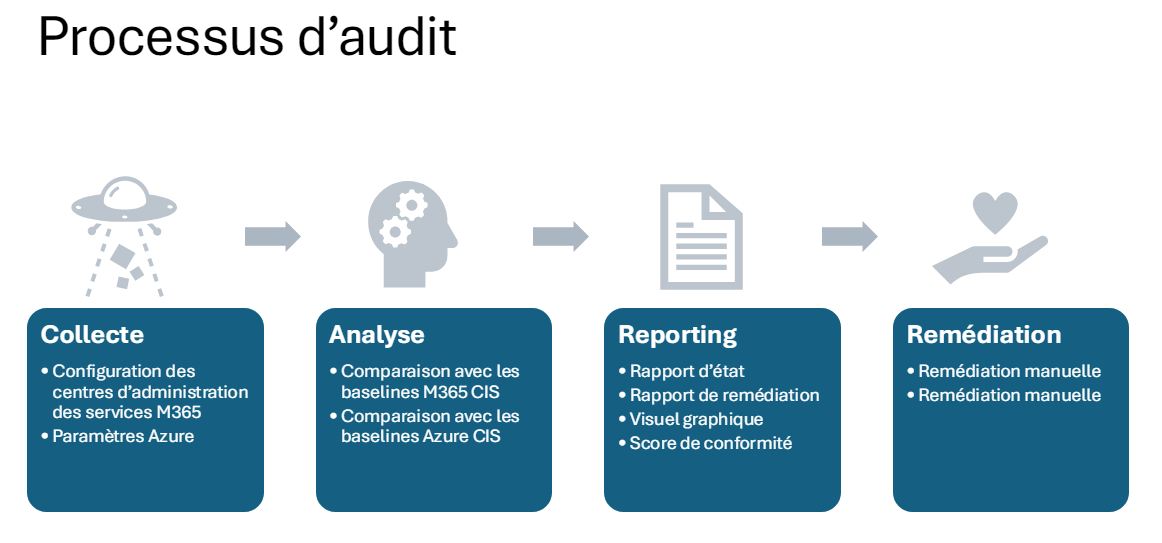
\includegraphics[scale=0.6]{images/ProcessusAudit.png}}
        \caption{Processus d'audit}
    \end{center}
\end{figure}

Ce schéma montre le flux complet du processus d'audit, incluant la collecte des configurations des services \textbf{M365}, l'analyse comparative avec les baselines \textbf{M365 CIS}( Center for Internet Security ) et \textbf{Azure CIS}, le reporting sous forme de rapports d'état et de remédiation, et enfin, la remédiation manuelle des écarts identifiés. Ce processus vise à garantir une meilleure efficacité et précision des audits, répondant ainsi aux objectifs principaux du projet.

\subsection{Étapes clés}

Le projet se déroulera en plusieurs phases principales :
\begin{itemize}
    \item[1.] \textbf{Phase de cadrage fonctionnel} : Identification des besoins, analyse des exigences et définition des User Stories.
    \item[2.] \textbf{Phase de développement} : Création de l'interface web d'administration en utilisant des technologies telles que \textbf{Microsoft .NET}, \textbf{Azure}, \textbf{M365} et \textbf{PowerShell}.
    \item[3.] \textbf{Phase de tests et validation} : Réalisation des tests unitaires, des tests d'intégration et des tests de régression pour garantir la qualité et la fiabilité de la solution.
    \item[4.] \textbf{Phase de déploiement} : Mise en production de l'application, optimisation des performances et formation des utilisateurs finaux.
    \item[5.] \textbf{Phase de suivi et d'amélioration continue} : Analyse des retours utilisateurs, correction des anomalies et mise à jour de l'application en fonction des besoins évolutifs.
\end{itemize}

\subsection{Méthodologie de travail}
Pour assurer une progression structurée et efficace du projet, une méthodologie de travail bien définie a été mise en place. Celle-ci repose sur plusieurs éléments clés. 

Des points de suivi sont organisés deux fois par semaine avec l'équipe, chaque mardi et jeudi. Ces réunions permettent de faire le point sur l'avancement du projet, de débloquer d'éventuelles difficultés, et d'assurer un suivi rigoureux de la progression.

Un tableau Kanban est utilisé sur Microsoft \textbf{Planner} pour la gestion des tâches. Ce tableau permet de visualiser les différentes étapes du projet et les tâches associées, facilitant ainsi la répartition du travail et le suivi de l'avancement. Chaque tâche est attribuée aux membres de l'équipe en fonction de leurs compétences et disponibilités.

Ci-dessous, une image du tableau Kanban utilisé, illustrant les différents types de tâches et leur répartition :

\begin{figure}[H]
    \begin{center}
        \fbox{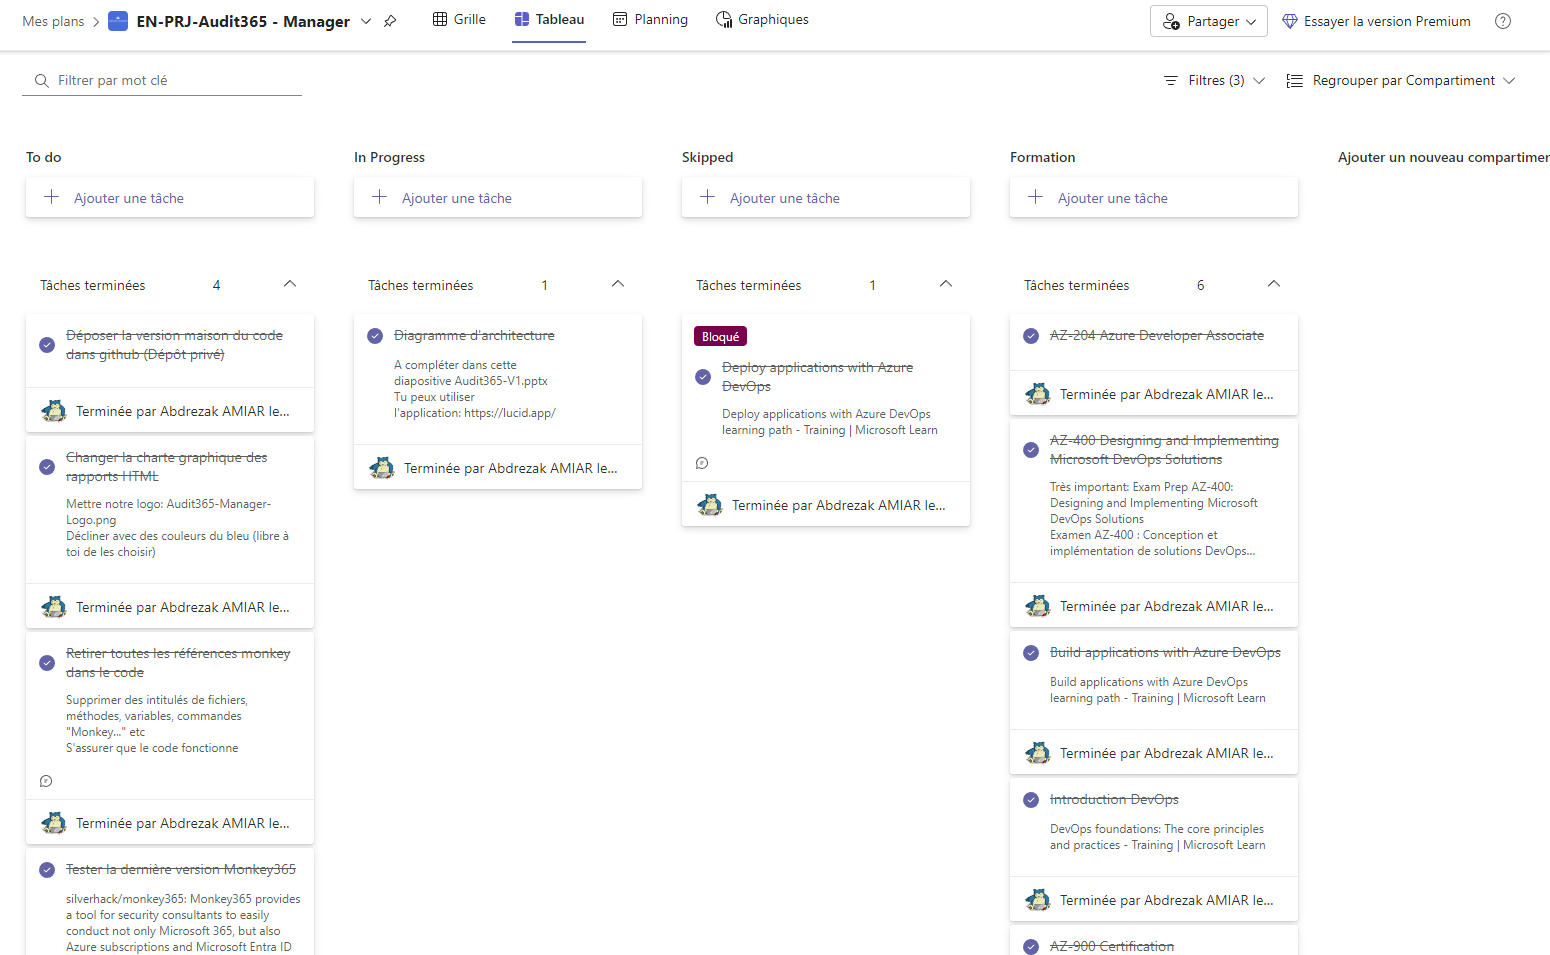
\includegraphics[scale=0.45]{images/TabPlanner.png}}
        \caption{Tableau Kanban sur Microsoft Planner}
    \end{center}
\end{figure}

Cette méthodologie de travail collaborative et visuelle permet de maintenir une communication fluide et une organisation claire, garantissant ainsi l'atteinte des objectifs du projet de manière efficace et structurée.

\section{Benchmark des solutions disponibles}
\subsection{Définition de Benchmark}

Dans le contexte de notre projet, le benchmarking consiste à comparer les solutions existantes d'audit et de gouvernance des \textbf{SI M365}. En analysant les fonctionnalités, les performances et les résultats obtenus par ces solutions, nous pouvons évaluer leur efficacité et identifier les points forts et les lacunes de notre propre solution. Cette démarche nous aide à définir des objectifs clairs et ambitieux, tout en garantissant que notre solution répond aux attentes élevées du marché et des utilisateurs finaux.

\subsection{Exemples de notre cas}

Pour illustrer le benchmarking dans le contexte de notre projet, nous avons analysé plusieurs solutions existantes d'audit et de gouvernance des \textbf{SI M365}. Voici quelques exemples de ces solutions :

\subsubsection{Microsoft365DSC}

Microsoft365DSC est une solution open source qui permet de gérer et de configurer les paramètres de \textbf{M365} de manière déclarative. Elle utilise des scripts PowerShell pour déployer et auditer les configurations, facilitant ainsi la gestion de la conformité et des changements dans l'environnement \textbf{M365}.

\begin{figure}[H]
    \begin{center}
        \fbox{
\includegraphics[scale=0.25]{images/M365DSC.png}}
        \caption{Logo Microsoft365DSC}
    \end{center}
\end{figure}
\vspace{-0.4cm}
\subsubsection{Monkey365}

Monkey365 est un outil spécialisé dans l'audit et la surveillance des environnements \textbf{M365} et \textbf{Azure}. Il offre des fonctionnalités avancées pour la collecte et l'analyse des données de configuration, permettant aux administrateurs de suivre les modifications et de garantir la conformité aux politiques de sécurité.

\begin{figure}[H]
    \begin{center}
        \fbox{
\includegraphics[scale=0.18]{images/monkey365.png}}
        \caption{Logo Monkey365}
    \end{center}
\end{figure}
\vspace{-0.4cm}
\subsubsection{Maester}

Maester est un outil de gouvernance et d'audit pour \textbf{Azure}, conçu pour simplifier la gestion des configurations et la conformité. Il offre des fonctionnalités pour l'audit des modifications, la gestion des permissions et l'analyse des configurations, aidant ainsi les administrateurs à gérer efficacement leurs environnements Cloud.

\begin{figure}[H]
    \begin{center}
        \fbox{
\includegraphics[scale=0.08]{images/maester.png}}
        \caption{Logo Maester}
    \end{center}
\endfigure}
\vspace{-0.4cm}
\subsubsection{EasyGovernance}

EasyGovernance est une plateforme qui propose des solutions de gouvernance pour \textbf{M365}. Elle inclut des modules pour l'audit, la gestion des accès et des permissions, ainsi que la conformité réglementaire. EasyGovernance aide les organisations à maintenir un contrôle strict sur leurs environnements \textbf{M365}.

\subsection{Résultat du Benchmark}

Après avoir analysé plusieurs solutions, nous avons sélectionné l'application de référence la plus alignée à nos besoins : \textbf{MONKEY365}. Voici les conclusions tirées de notre benchmark :
\begin{itemize}
\item[•] \textbf{Microsoft365DSC} est une solution très avancée qui permet de gérer et configurer les paramètres de Microsoft 365 de manière déclarative. Cependant, sa complexité et ses nombreuses fonctionnalités dépassent largement nos besoins actuels, rendant cette solution surdimensionnée pour notre projet.

\item[•] \textbf{EasyGovernance} propose des fonctionnalités de gouvernance pour \textbf{M365}, mais elle est encore en développement. Elle présente plusieurs bugs et certaines de ses fonctionnalités ne fonctionnent que partiellement, ce qui la rend moins fiable pour notre utilisation.

\item[•] \textbf{Maester} est une solution efficace pour la gouvernance et l'audit, mais elle se concentre uniquement sur la partie \textbf{Azure}. Étant donné que notre projet se concentre sur les deux environnements \textbf{M365} et \textbf{Azure}, cette solution ne répond pas entièrement à nos besoins actuels.

\item[•] \textbf{MONKEY365} est la solution qui se rapproche le plus de nos objectifs. Elle offre des fonctionnalités avancées pour l'audit et la surveillance des environnements \textbf{M365} et \textbf{Azure}, ce qui correspond parfaitement à nos besoins. Sa capacité à collecter et analyser les données de configuration, ainsi que sa fiabilité et sa conformité aux politiques de sécurité, en font l'application de référence idéale pour notre projet.
\end{itemize}
\vspace{0.1cm}
Ainsi, \textbf{MONKEY365} a été sélectionnée comme l'application de référence alignée à nos besoins, nous permettant d'atteindre nos objectifs de manière efficace et fiable.

\section{Étude Conceptuelle}

\subsection{Nos besoins}

Pour mener à bien le projet \textbf{Audit365 Manager}, il est crucial de bien définir les besoins spécifiques. Ces besoins seront articulés autour de deux aspects principaux : les personas et les user stories, qui permettent de comprendre les utilisateurs cibles et les fonctionnalités attendues.

\subsubsection{Personas}

Les personas représentent les profils types des utilisateurs finaux de notre solution. Ils aident à mieux cerner leurs attentes, leurs objectifs et leurs comportements. Voici quelques exemples de personas identifiés pour notre projet :

\begin{itemize}
    \item \textbf{Auditeur général} : Responsable de la surveillance et de l'évaluation de l'ensemble des services et fonctionnalités de la plateforme \textbf{M365}. Son objectif est de s'assurer que les politiques et les normes de l'organisation sont respectées.
    \item \textbf{Auditeur des services SharePoint} : Spécialisé dans la surveillance des environnements SharePoint Online. Il veille à ce que les sites, les bibliothèques de documents et les permissions respectent les normes de l'organisation. (Persona Visé pour notre V1)
    \item \textbf{Auditeur des services de collaboration Teams} : Chargé d'assurer le bon fonctionnement des fonctions de collaboration dans Teams. Il surveille la gestion des canaux, des équipes et des politiques associées.
\end{itemize}

\subsubsection{User stories}

Les user stories sont des descriptions simples et concises des fonctionnalités que les utilisateurs finaux souhaitent obtenir. Elles sont formulées du point de vue de l'utilisateur et servent de base pour le développement des fonctionnalités. Voici quelques user stories pour notre projet :

\begin{table}[h!]
\begin{center}
\begin{tabular}{| m{0.2\textwidth} | m{0.75\textwidth} |}
\hline
\textbf{Catégorie} & \textbf{User Story} \\
\hline
\textbf{Collecte} & En tant qu'auditeur des services SharePoint, je souhaite avoir accès à un backoffice pour configurer les paramètres de collecte de données de SharePoint afin de m'assurer que toutes les configurations nécessaires sont correctement auditées. \\
\hline
\textbf{Analyse} & En tant qu'auditeur des services SharePoint, je souhaite comparer les configurations collectées avec les baselines M365 CIS afin d'identifier les écarts de conformité spécifiques à SharePoint. \\
\hline
\textbf{Reporting} & En tant qu'auditeur des services SharePoint, je souhaite générer des rapports d'état détaillés sur la conformité de SharePoint afin de fournir une vue claire de la posture de sécurité et des domaines nécessitant des améliorations. \\
\hline
\textbf{Remédiation} & En tant qu'auditeur des services SharePoint, je veux pouvoir effectuer des remédiations manuelles ou automatiques des écarts de conformité identifiés afin de corriger les configurations de sécurité de SharePoint. \\
\hline
\textbf{Backoffice} & En tant qu'auditeur des services SharePoint, je souhaite configurer les paramètres d'audit tels que les services spécifiques à auditer via le backoffice afin de m'assurer que les audits sont effectués de manière ciblée. \\
\hline
\end{tabular}
\caption{User Stories}
\end{center}
\end{table}

Ces personas et user stories permettent de structurer le développement du projet en se concentrant sur les besoins réels des utilisateurs, garantissant ainsi une solution efficace et adaptée.

\subsection{Référentiels des normes de sécurité (Security Framework)}

Pour assurer la conformité et la sécurité des \textbf{SI M365}, il est essentiel de se baser sur des référentiels de normes de sécurité reconnus, souvent nommés "Baselines". Ces référentiels fournissent des lignes directrices et des meilleures pratiques pour garantir que les configurations et les opérations des \textbf{SI} répondent aux exigences de sécurité et de conformité. Parmi les principaux référentiels utilisés, nous avons :

\textbf{CIS (Center for Internet Security)} : Le CIS propose des benchmarks et des guidelines de sécurité spécifiques à différents environnements, dont \textbf{M365} et \textbf{Azure}. Ces benchmarks fournissent des configurations de sécurité recommandées pour protéger contre les menaces courantes et assurer la conformité aux meilleures pratiques de sécurité. Dans notre projet, nous avons décidé d'utiliser le référentiel CIS comme référence principale, car il est le plus conforme à nos besoins. Toutefois, il est possible que nous fassions des ajustements en fonction des situations spécifiques, tout en conservant CIS comme notre première référence.

\textbf{SCuBA (Secure Cloud Business Applications)} : SCuBA est un ensemble de recommandations et de pratiques pour sécuriser les applications cloud. Il propose des solutions pour gérer les risques de sécurité liés à l'utilisation des services cloud, en mettant l'accent sur la protection des données et la gestion des accès.

\textbf{BluePrint} : BluePrint offre des modèles et des configurations sécurisées pour divers services \textbf{M365} et \textbf{Azure}. Il aide à déployer des environnements conformes aux normes de sécurité, facilitant ainsi la mise en place de mesures de protection robustes et cohérentes.

En plus de ces référentiels, il existe d'autres normes et frameworks de sécurité, tels que NIST (National Institute of Standards and Technology), ISO/IEC 27001, et GDPR (General Data Protection Regulation), qui peuvent être utilisés pour renforcer la sécurité et la conformité des systèmes d'information. Ces référentiels fournissent des lignes directrices supplémentaires pour la gestion des risques, la protection des données et la gouvernance des \textbf{SI}.

L'adoption de ces référentiels de sécurité permet de garantir que notre solution \textbf{Audit365 Manager} est alignée avec les meilleures pratiques de l'industrie, assurant ainsi une protection optimale des environnements \textbf{M365} et \textbf{Azure}.

\section{Récapitulatif}

\textit{Ce chapitre a permis de définir le périmètre du projet \textbf{Audit365 Manager}. Nous avons examiné le contexte, les objectifs principaux, les étapes clés, et la méthodologie de travail. Un benchmark des solutions existantes a été réalisé, menant à la sélection de MONKEY365 comme application de référence. Enfin, une étude conceptuelle a été menée pour définir les besoins et les référentiels de sécurité.}

\textit{Le prochain chapitre traitera du cadrage technique du projet.}


